\documentclass[a4paper]{article}

\usepackage[T1]{fontenc}
\usepackage[utf8]{inputenc}
\usepackage[italian]{babel}
\usepackage{frontespizio}
\usepackage{graphicx}

\begin{document}
	
	
\begin{frontespizio} 
 \Preambolo{\renewcommand{\frontpretitlefont}{\fontsize{14}{12}\scshape}}
\Universita{Pisa} 
\Facolta{Ingegneria} 
\Corso[Laurea]{Ingegneria Informatica} 
\Annoaccademico{2019--2020} 
\Titolo{Titolo} 
\Sottotitolo{Sottotitolo}
\Filigrana [height=4cm,before=0.28,after=1]{./images/stemma_unipi.png} 


\Rientro{1cm} 
\Candidato{Marco Parola} 
\Relatore{Dr. Francesco Pistolesi}
\Punteggiatura{} 
 
\end{frontespizio}

	\tableofcontents

	\clearpage



	\section{Introduzione}
Lo scopo di questa tesi è analizzare i movimenti compiuti durante il sollevamento di un carico elevato mediante dispositivi indossabili che contengono al loro interno sensori. \\
L’utilità di questo tipo di analisi diventa evidente quando andiamo a considerare i dati provenienti dagli enti di previdenza sociale relativi al tipo e ai numeri degli infortuni sul lavoro e delle malattie professionali. Questi dati evidenziano infatti come, a livello mondiale, a prevalere siano malattie professionali classificabili come disturbi Muscolo-Scheletrici. \\
La mansione del sollevamento di un carico aumenta in maniera considerevole l'indice di rischio di questo tipo di disturbi.
Considerando poi che quasi un terzo dei lavoratori dichiara di svolgere quotidianamente questo tipo di operazione, è lecito pensare che avendo uno strumento capace di analizzare il modo in cui si effettua questo task potrebbe permettere di comprendere il problema più a fondo e cercare una soluzione mirata.

	\clearpage

	\section{Movimentazione corretta e scorretta per il sollevamento di un carico}
L'operazione di sollevamento di un carico...


	\clearpage

	\section{Raccolta dati}
Per poter eseguire uno studio del rischio che corre una persona, sollevando un carico elevato, si affronta una prima fase in cui si raccolgono i dati relativi alla movimentazione di quest'ultima. \\
Dunque si rende necessario uno strumento che permetta di raccogliere e catalogare informazioni con cui poter ricostruire il movimento ed in una seconda fase eseguire un analisi per poter quantificare il rischio. \\



	\subsection{Sistema per la raccolta ed il salvataggio di dati}


	\subsubsection{Caratteristiche}
Il sistema di cui ci muniremo dovrà contenere al suo interno sensori di vario genere, che gli permettano di registrare i movimenti e le variazioni delle condizioni ambientali esterne a cui è sottoposto, i sensori che prenderemo in considerazione e di cui l'hardware che useremo deve essere munito sono i seguenti:
\begin{itemize}
\item Accelerometro triassiale, misura l’accelerazione che subisce il dispositivo sui tre assi cardinali.
\item Giroscopio triassiale, misura la velocità angolare del dispositivo attorno ai tre assi del sistema di riferimento.
\item Magnetometro triassiale, misura l’intensità del flusso del campo magnetico terrestre relativamente ai tre assi del sistema di riferimento. Tramite questo tipo di sensore possiamo ricavare informazioni sull’angolo che questo dispositivo forma con il campo magnetico terrestre.
\item Barometro, misura la pressione atmosferica alla quale il dispositivo è sottoposto; grazie alla elevata sensibilità di questo sensore è possibile individuare variazioni di pressione anche molto piccole, dell’ordine dei mbar.
\end{itemize}
Inoltre un'altra proprietà che il nostro sistema deve possedere è essere \textbf{miniinvasivo}, infatti la persona che utilizza uno strumento di questo tipo non dovrebbe quasi accorgersi della sua esistenza, affinché non si senta eccessivamente controllato, oppure disturbato nei movimenti che compie.

	\subsubsection{Applicazione Android per la rccolta}
La soluzione che abbiamo trovato, che rispecchia i requisiti di sopra riportati è un'applicazione Android composta da due moduli, uno che girerà su smartphone e una su smartwatch.

	\subsection{Esperimenti di registraione}
Dopo essersi muniti di uno strumento che rispecchi i requisiti precedentemente elencati, si  affronta una fase in cui si eseguono uno o più esperimenti di registrazione: ogni esperimento è definito da un set di azioni, che dovranno essere svolte da un candidato, mentre il sistema di registrazione e salvataggio dei dati memorizza tutte le informazioni neccessarie a ricostruire la movimentazione compiuta.

	\subsubsection{Esperimento 1}
Il primo esperimento da svolgere è molto semplice, vengono eseguite essenzialmente 3 azioni: camminata, sollevamento, abbassamento.
La ultime due azioni possono essere fatte in maniera sicura oppure dannosa per la schiena.
Di seguito è riportato uno schema del modulo:\\

\begin{center}
    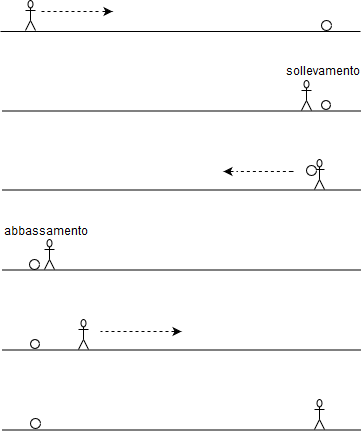
\includegraphics[width=60mm,scale=0.7]{./images/esperimento1.png} 
\end{center} 

Questo schema riassume un ciclo del percorso totale. L’esperimento completo prevederà N cicli, di cui N/2 in cui il sollevamento/abbassamento viene eseguito correttamente, N/2 scorrettamente.

	\subsubsection{Esperimento 2}
Di seguito verrà presentato il modulo delle azioni svolte, in cui si simulano alcune manovre che un operaio può compiere durante la giornata lavorativa:
\begin{itemize}
\item 5 secondi, raccogliere un oggetto leggero da terra
\item 50 secondi,  utilizzo dello smartphone in posizione eretta 
\item 10 secondi, dirigersi verso l’oggetto da sollevare e compiere il sollevamento corretto
\item 20 secondi, camminare
\item 30 secondi, accucciarsi e simulare una mansione di lavoro su un oggetto posto in basso
\item 10 secondi, dirigersi verso l’oggetto e compiere il sollevamento scorretto
\item 10 secondi, dirigersi verso una scrivania e sedersi alla postazione di lavoro
\item 50 secondi, lettura e/o utilizzo del computer
\item 5 secondi, raccogliere un oggetto leggero da terra
\item 15 secondi, dirigersi verso l’oggetto e compiere due volte il sollevamento corretto
\item 50 secondi, simulare l’azione di dare il cencio e/o la scopa
\item 15 secondi, compiere due volte il sollevamento scorretto
\end{itemize}
Durata: 4.30 minuti \\
Sollevamenti: 8 sollevamenti (2 leggeri, 3 corretti, 3 scorretti)



\end{document}




